\documentclass[12pt]{article}
\usepackage{amsmath,amsthm,amssymb,amsfonts,setspace,xfrac,graphicx}

\textwidth 7.0 truein
\oddsidemargin -0.25in   %left-hand edge
\evensidemargin -0.5 truein  %right-hand edge
\topmargin -0.85in      %top of paper to top of head, pulls whole unit
\textheight 9.5in

%%%% In most cases you won't need to edit anything above this line %%%%

\begin{document}
\hfill Tanner Kvarfordt

\hfill A02052217

\hfill Math 2270

\hfill Assignment \#6


\begin{itemize}
\item[3.4.16)] Find a basis for each of these subspaces of $\mathbb{R}^4$:
\begin{itemize}
\item[a)] All vectors whose components are equal.
\item[b)] All vectors whose components add to zero.
\item[c)] All vectors that are perpendicular to $(1,1,0,0)$ and $(1,0,1,1)$.
\item[d)] The column space and the nullspace of $I$ (4 by 4).
\end{itemize}

\textit{Solution.}
\begin{itemize}
\item[a)] Let $S$ denote the subspace of $\mathbb{R}^4$ where all vectors have components that are equivalent. Consider the set of vectors, $\{ \vec{w}\}$ where $\vec{w}=(1,1,1,1)$. $\vec{w}$ is clearly linearly independent since it is the only vector, so if it is also a spanning set of $S$, then it is a basis of $S$. $S$ has the form $(a,a,a,a)$. Consider that $c_1\vec{w}=(a,a,a,a)$ shows that $c_1=a$. Therefore $\{\vec{w}\}$ is a spanning set of $S$. Hence $\{\vec{w}\}$ is a basis of $S$.
\item[b)] Let $S$ denote the subspace of $\mathbb{R}^4$ where all vectors have components that sum to $0$. Consider the set of vectors $\{\vec{w}, \vec{u}, \vec{v}\} = \{(1,-1,0,0),(1,0,-1,0),(1,0,0,-1)\}$. Consider the $m \times n$ matrix
$\left[\begin{array}{ccc} \vec{w} & \vec{u} & \vec{v}\end{array}\right]$. Performing elimination on this matrix gives 
$\left[\begin{array}{ccc}
1 & 1 & 1\\ 
0 & 1 & 1\\
0 & 0 & 1\\
0 & 0 & 0
\end{array}\right]$. Since there are $n$ pivots, the three column vectors are linearly independent. It then follows that if $\vec{w}$, $\vec{u}$, and $\vec{v}$ form a spanning set of $S$, then they are a basis of $S$. $S$ has the form $(a,b,c,d)$ where $a+b+c+d=0$. Consider that $c_1\vec{w}+c_2\vec{u}+c_3\vec{v}=(c_1+c_2+c_3,-c_1,-c_2,-c_3)$ and thus is in $S$. Therefore $\{\vec{w}, \vec{u}, \vec{v}\}$ is a spanning set of $S$, and thus is also a basis of $S$.

\item[c)] Let $S$ denote the subspace of $\mathbb{R}^4$ where all vectors are perpendicular to  $(1,1,0,0)$ and $(1,0,1,1)$, thus $S$ has the form $(a,b,c,d)$ where $a+b=0$ and $a+c+d=0$.\\
Consider the set of vectors $\{\vec{w}, \vec{u}\} = \{(1,-1,-1,0),(1,-1,0,-1)\}$. Consider the $m \times n$ matrix
$\left[\begin{array}{cc} \vec{w} & \vec{u}\end{array}\right]$. Performing elimination on this matrix gives 
$\left[\begin{array}{cc}
1 & 1 \\ 
0 & 1 \\
0 & 0 \\
0 & 0
\end{array}\right]$. Since there are $n$ pivots, the three column vectors are linearly independent. It then follows that if $\vec{w}$ and $\vec{u}$ form a spanning set of $S$, then they are a basis of $S$. Consider that $c_1\vec{w}+c_2\vec{u}=(c_1+c_2,-c_1-c_2,-c_1,-c_2)$ and thus is in $S$ since the result fits the form described above. Therefore $\{\vec{w}, \vec{u}\}$ is a spanning set of $S$, and thus is also a basis of $S$.
\item[d)] Because the pivot columns of any matrix form a basis of its column space, the column vectors of $I$ are a basis of C$(I)$. Because N$(I)=$ span$\{\vec{0}\}$, the $\{0,0,0,0\}$ is the basis of N$(I)$.
\end{itemize}

\item[3.4.24)] True or false:
\begin{itemize}
\item[a)] If the columns of a matrix are dependent, so are the rows.
\item[b)] The column space of a 2 by 2 matrix is the same as its row space.
\item[c)] The column space of a 2 by 2 matrix has the same dimension as its row space.
\item[d)] The columns of a matrix are a basis for the column space.
\end{itemize}

\textit{Solution.}
\begin{itemize}
\item[a)] False. Consider the matrix $\left[\begin{array}{ccc} 12 & 12 & 12 \end{array}\right]$. The three columns are clearly dependent, but there is only one row, and therefore the single row vector must be independent.
\item[b)] False. Consider the matrix $A=\left[\begin{array}{cc} 1 & 2 \\ 1 & 2\end{array}\right]$. C($A$)$=$span$\{\left[\begin{array}{c} 1 \\ 1\end{array}\right]\}$ $\neq$ 
C($A^T$)=span$\{\left[\begin{array}{c} 1 \\ 2\end{array}\right]\}$
\item[c)] True. Both are equivalent to the rank of the matrix.
\item[d)] False. Some matrices may not have linearly independent column vectors.
\end{itemize}

\item[3.5.13)] True or False:
\begin{itemize}
\item[a)] If $m=n$ then the row space of $A$ equals the column space.
\item[b)] The matrices $A$ and $-A$ share the same four subspaces.
\item[c)] If $A$ and $B$ share the same four subspaces then $A$ is a multiple of $B$.
\end{itemize}

\textit{Solution.}
\begin{itemize}
\item[a)] False. See my answer to problem 3.4.24 part b for a counterexample.
\item[b)] True. The four subspaces will be spans of vectors that can be written as linear combinations of each other.
\item[c)] False. Consider $A=\left[\begin{array}{cc} 1 & 0 \\ 0 & 2\end{array}\right]$ and 
$B=\left[\begin{array}{cc} 2 & 0 \\ 0 & 1\end{array}\right]$. They are both invertible 2 by 2 matrices, and therefore have the same four subspaces, but are clearly not multiples of each other.
\end{itemize}

\item[4.1.17)] 
\begin{itemize}
\item[a)] If $S$ is the subspace of $\mathbb{R}^3$ containing only the zero vector, what is $S^\perp$?
\item[b)] If $S$ is spanned by $(1,1,1)$, what is $S^\perp$?
\item[c)] If $S$ is spanned by $(1,1,1)$ and $(1,1,-1)$, what is a basis for $S^\perp$
\end{itemize}

\textit{Solution.}
\begin{itemize}
\item[a)] Since $S$ contains only $\vec{0}$, $\vec{v}_1\vec{0}$ is in $S$ for any $c_1$. Since anything dotted with $\vec{v}$ produces 0, $S^\perp = \mathbb{R}^3$
\item[b)] $S^\perp$ is the plane spanned by any two linearly independent vectors perpendicular to $(1,1,1)$ such as $(1,0,-1)$ and $(0,1,-1)$. For proof, consider \\
$[c_1(1,0,-1) + c_2(0,1,-1)] \cdot c_3(1,1,1)= c_3(1,1,1) \cdot c_1(1,0,-1) + c_3(1,1,1) \cdot c_2(0,1,-1)=\vec{0}$\\
As well as the fact that dim$[S] +$ dim$[$span$\{(1,0,-1),(0,1,-1)\}$ $]=3=$ dim$[\mathbb{R}^3]$ 
\item[c)] Since we know that the sum of the dimensions of each subspace must be three, we know we $S^\perp$ has dimension $1$. So $S^\perp =$ span$\{\vec{v}\}=$ span$\{(1,-1,0)\}$, where $\vec{v}$ can be found by solving
$\vec{v} \cdot [(1,1,1) + (1,1,-1)] = \vec{0}$. To cement the proof that $S^\perp =$ span$\{(1,-1,0)\}$ (note we already know that the dimensions add up properly), see that\\
$[c_1(1,1,1) + c_2(1,1,-1)] \cdot c_3(1,-1,0)= c_3(1,-1,0) \cdot c_1(1,1,1) + c_3(1,-1,0) \cdot c_2(1,1,-1)=\vec{0}$
I also claim that $\{\vec{v}\}$ is a basis for $S^\perp$. $S^\perp$ has the form $(m,-m,0)$. See that 
$k(1,-1,0)=(m,-m,0)$ where $k=m$, and since $\vec{v}$ is the only vector in the set, it is linearly independent.
\end{itemize}

\item[S1)] Find the dimensions and bases for the four fundamental subspaces of $\mathbf{A}=\left[\begin{array}{cccc} 1 & 2 & 3 & 2\\ 2 & 5 & 7 & 6\\ 4 & 6 & 10 &4\end{array}\right]$.  \\ 

\textit{Solution.}
\[\mathbf{A}=\left[\begin{array}{cccc} 1 & 2 & 3 & 2\\ 2 & 5 & 7 & 6\\ 4 & 6 & 10 &4\end{array}\right]
 \underset{E_{1} \text{ where } -l_{21}=-2 \text{ and }-l_{31}=-4}{\xrightarrow{\hspace{40mm}}}
 \left[\begin{array}{cccc} 1 & 2 & 3 & 2\\ 0 & 1 & 1 & 2\\ 0 & -2 & -2 & -4\end{array}\right]\]
 \[\underset{E_{32} \text{ where } -l_{32}=-1}{\xrightarrow{\hspace{30mm}}}
 \left[\begin{array}{cccc} 1 & 2 & 3 & 2\\ 0 & 1 & 1 & 2\\ 0 & 0 & 0 & 0\end{array}\right] = U\]
\begin{itemize}
	\item[i)] dim[C$(A)$]$=2$; basis of C$(A)=\{(1,2,4),(2,5,6)\}$
    \item[ii)] dim[C$(A^T)$]$=2$; basis of C$(A^T)=\{(1,2,3,2),(2,5,7,6)\}$
    \item[iii)] dim[N$(A)$]$=2$; Solve $U\vec{x}=\vec{0}$ by setting the first free variable $x_3=1$ and the second free variable $x_4=0$, and then $x_3=0$ and $x_4=1$ to get the basis of N$(A)=\{(2,-2,0,1),(-1,-1,1,0)\}$
    \item[iv)] dim[N$(A^T)$]$=1$; basis of N$(A^T)$ is the free rows of $A$ in $E$ where 
    \[E=E_{32}E_{1}=\left[\begin{array}{ccc} 1 & 0 & 0\\ -2 & 1 & 0 \\ -8 & 2 & 1\end{array}\right]\] and therefore a basis of N$(A^T)=\{(-8,2,1)\}$
	\end{itemize}

\item[S2)]
\begin{itemize}
\item[a)] Let $\mathbf{A}$ be a 4x7 matrix.  What is the largest dimension for the nullspace of $\mathbf{A}$? What is the smallest dimension for the nullspace of $\mathbf{A}$?
\item[b)] Let $\{\vec{v}_1,...,\vec{v}_n\}$ and $\{\vec{w}_1,...,\vec{w}_n\}$ be bases of the vector space $\mathcal{V}$.  What are the dimensions of $\mathcal{V}$, span$(\{\vec{v}_1,...,\vec{v}_n\})$ and span$(\{\vec{w}_1,...,\vec{w}_n\})$?
\end{itemize}

\textit{Solution.}
\begin{itemize}
\item[a)] $A$ is $m \times n$. dim[N$(A)$]$=n -$rank$(A)$. Since $0 \leq$ rank$(A) \leq 4$ in this case, 
	$3 \leq$ dim[N$(A)$] $\leq 7$.
\item[b)] Because the two sets contain $n$ vectors each (implying each spanning set has dimension $n$), the dimension of $\mathcal{V}$ is $2n$. 
\end{itemize}


\item[S3)] This problem focuses on finding bounds for the rank of a matrix when it is the product of other matrices.  
\begin{itemize}
\item[a)] Consider $A = \left[\begin{array}{ccc}  1 & 1\\ 1  & 1\end{array}\right]$ and $B= \left[\begin{array}{ccc}2 & 3\\ 1 & 1 \end{array}\right]$.  Compute the ranks of $A$, $B$, $AB$, and $BA$.
\item[b)] Based on your answer to part (a), come up with lower and upper bounds for rank$(AB)$ and rank($BA$) that depend on the values of rank($A$) and rank($B$). 
\item[c)] Now consider $C=\left[\begin{array}{cc} 0 & 0\\ 0 &1 \end{array}\right]$ and $D=\left[\begin{array}{cc} 1 & 0\\ 0 &0 \end{array}\right]$.  Compute the ranks of $C$, $D$, $CD$ and $DC$.
\item[d)] Based on the answers to (a) and (c), revise your upper and lower bounds from part (b).
\end{itemize}

\textit{Solution.}
\begin{itemize}
\item[a)] 
	\begin{itemize}
	\item[i)] $A = \left[\begin{array}{ccc} 1 & 1\\ 1 & 1\end{array}\right]
    		  \underset{E_{21} \text{ where } -l_{21}=-1}{\xrightarrow{\hspace{30mm}}}
              \left[\begin{array}{ccc} 1 & 1\\ 0  & 0\end{array}\right] \Rightarrow$ r$(A)=1$
    \item[ii)] $B = \left[\begin{array}{ccc} 2 & 3\\ 1  & 1\end{array}\right]
    		  \underset{E_{21} \text{ where } -l_{21}=\sfrac{-1}{2}}{\xrightarrow{\hspace{30mm}}}
              \left[\begin{array}{ccc} 2 & 3\\ 0 & \sfrac{-1}{2}\end{array}\right] \Rightarrow$ r$(B)=2$
    \item[iii)] $AB = \left[\begin{array}{ccc} 3 & 4\\ 3  & 4\end{array}\right]
    		  \underset{E_{21} \text{ where } -l_{21}=-1}{\xrightarrow{\hspace{30mm}}}
              \left[\begin{array}{ccc} 3 & 4\\ 0 & 0\end{array}\right] \Rightarrow$ r$(AB)=1$
    \item[iv)] $BA = \left[\begin{array}{ccc} 5 & 5\\ 2  & 2\end{array}\right]
    		  \underset{E_{21} \text{ where } -l_{21}=\sfrac{-2}{5}}{\xrightarrow{\hspace{30mm}}}
              \left[\begin{array}{ccc} 5 & 5\\ 0 & 0\end{array}\right] \Rightarrow$ r$(BA)=1$
	\end{itemize}
\item[b)] Based on part (a), $r(AB)=r(A)$ and $r(BA)=r(A)$
\item[c)] \begin{itemize}
	\item[i)] $C = \left[\begin{array}{ccc} 0 & 0\\ 0 & 1\end{array}\right]
    		   \Rightarrow$ r$(C)=1$
    \item[ii)] $D = \left[\begin{array}{ccc}  1 & 0\\ 0  & 0\end{array}\right]
    		   \Rightarrow$ r$(D)=1$
    \item[iii)] $CD = \left[\begin{array}{ccc} 0 & 0\\ 0 & 0\end{array}\right]
    		  \Rightarrow$ r$(CD)=0$
    \item[iv)] $DC =\left[\begin{array}{ccc} 0 & 0\\ 0  & 0\end{array}\right]
    		   \Rightarrow$ r$(DC)=0$
	\end{itemize}
\item[d)] Based on parts (a) and (b), $0 \leq r(AB) \leq r(A)$ and $0 \leq r(BA) \leq r(A)$
\end{itemize}

\item[S4)] Find a basis and the dimension for each of the following subspaces of $M_{3\times3}$:
\begin{itemize}
\item[a)] All matrices spanned by the identity matrix. 
\item[b)] All matrices spanned by $\left\{\left[\begin{array}{ccc} 1 & 0 & 0\\ 0 & 0 &0 \\ 0& 0& 0\end{array}\right], \left[\begin{array}{ccc} 0 & 1 & 0\\ 0 & 0 & 0\\ 0& 0& 0\end{array}\right], \cdots, \left[\begin{array}{ccc} 0 & 0 & 0\\ 0 & 0 & 0\\ 0& 0& 1\end{array}\right]\right\}$
\item[c)] All symmetric matrices, i.e., matrices satisfying $A=A^\text{T}$
\end{itemize}

\textit{Solution.}
\begin{itemize}
\item[a)] Matrices spanned by the identity matrix have the form 
$\left[\begin{array}{ccc} x & 0 & 0 \\ 0 & y & 0 \\ 0 & 0 & z\end{array}\right]$, so my guess for a basis will be 
$\left\{ \vec{v_1}, \vec{v_2}, \vec{v_3} \right\} = \left\{
\left[\begin{array}{ccc} 1 & 0 & 0 \\ 0 & 0 & 0 \\ 0 & 0 & 0\end{array}\right], 
\left[\begin{array}{ccc} 0 & 0 & 0 \\ 0 & 1 & 0 \\ 0 & 0 & 0\end{array}\right],
\left[\begin{array}{ccc} 0 & 0 & 0 \\ 0 & 0 & 0 \\ 0 & 0 & 1\end{array}\right]\right\}$.
See that my guess for a basis is a spanning set because $c_1\vec{v_1} + c_2\vec{v_2}+ c_3\vec{v_3}=
\left[\begin{array}{ccc} x & 0 & 0 \\ 0 & y & 0 \\ 0 & 0 & z\end{array}\right]$ where $c_1=x$, $c_2=y$, and $c_3=z$.
Also, my guess for a basis is linearly independent since $c_1\vec{v_1} + c_2\vec{v_2}+ c_3\vec{v_3}=
\left[\begin{array}{ccc} 0 & 0 & 0 \\ 0 & 0 & 0 \\ 0 & 0 & 0\end{array}\right]$ only when $c_1=c_2=c_3=0$, thus proving that $\left\{ \vec{v_1}, \vec{v_2}, \vec{v_3} \right\}$ is a basis with dimension 3 of the subspace of $M_{3\times3}$ where all matrices are spanned by the identity matrix.
\item[b)] The basis would just be the set of the nine vectors of the spanning set, with dimension nine. They are a spanning set by definition of the problem, and they are all clearly linearly independent.
\item[c)] Symmetric $3 \times 3$ matrices have the form
$\left[\begin{array}{ccc} a & b & c \\ b & d & e \\ c & e & f\end{array}\right]$, so my guess for a basis will be
\[\left\{ \vec{v_1}, \vec{v_2}, \vec{v_3},\vec{v_4}, \vec{v_5}, \vec{v_6} \right\} = \] \[\left\{
\left[\begin{array}{ccc} 1 & 0 & 0 \\ 0 & 0 & 0 \\ 0 & 0 & 0\end{array}\right], 
\left[\begin{array}{ccc} 0 & 0 & 0 \\ 0 & 1 & 0 \\ 0 & 0 & 0\end{array}\right],
\left[\begin{array}{ccc} 0 & 0 & 0 \\ 0 & 0 & 0 \\ 0 & 0 & 1\end{array}\right],
\left[\begin{array}{ccc} 0 & 1 & 0 \\ 1 & 0 & 0 \\ 0 & 0 & 0\end{array}\right], 
\left[\begin{array}{ccc} 0 & 0 & 1 \\ 0 & 0 & 0 \\ 1 & 0 & 0\end{array}\right],
\left[\begin{array}{ccc} 0 & 0 & 0 \\ 0 & 0 & 1 \\ 0 & 1 & 0\end{array}\right] \right\}\]
See that my guess for a basis is a spanning set because \[c_1\vec{v_1} + c_2\vec{v_2}+ \cdots + c_6\vec{v_6}=
\left[\begin{array}{ccc} a & b & c \\ b & d & e \\ c & e & f\end{array}\right]\] where $c_1=a$, $c_2=d$, $c_3=f$, $c_4=b$, $c_5=c$, and $c_6=e$. Also, my guess for a basis is linearly independent since
\[c_1\vec{v_1} + c_2\vec{v_2}+ \cdots + c_6\vec{v_6}=
\left[\begin{array}{ccc} 0 & 0 & 0 \\ 0 & 0 & 0 \\ 0 & 0 & 0\end{array}\right]\] only when $c_1=c_2=\cdots=c_6=0$, thus proving that $\left\{ \vec{v_1}, \vec{v_2}, \vec{v_3},\vec{v_4}, \vec{v_5}, \vec{v_6} \right\}$ is a basis with dimension 6 of the subspace of $M_{3\times 3}$ where all matrices are symmetric.
\end{itemize}

\item[S5)] Take a deep breath.  In this problem, you will work with polynomials of degree at most 2, e.g., $1+4x+3x^2$. I want to you think about these polynomials in new way: as vectors.  We do this by writing the polynomial $a+bx+cx^2$ as the vector $(a,b,c)^T$.  That is, the first coordinate in the vector is the coefficient of the constant term ($a$); the second coordinate in the vector is the coefficient of the linear term ($b$); and the third coordinate in the vector is the coefficient of the quadratic term ($c$).  In this representation, the polynomial $\pi+ex-3x^2$ is the vector $(\pi,e,-3)^T$.  

Consider the polynomials $c(x)=1$, $l(x)=x$, and $q(x)=x^2$.  These polynomials are the vectors $(1,0,0)^T$, $(0,1,0)^T$, and $(0,0,1)^T$. The span of those vectors is the subspace $\mathcal{P}_2=\textsf{span}\{1,x,x^2\}$, i.e, the polynomials of degree at most 2.  This span contains the vectors $2+x+3x^2$, $\pi + x^2$, $x - ex^2$, $-x^2$, etc.   If we take the derivative of a polynomial $p(x) =c+bx+a^2$, we get $p'(x)=b+2ax$.  Notice that the original polynomial and the derivative are vectors, specifically $(c,b,a)^T$ and $(b,2a,0)^T$. 

\begin{itemize}
\item[a)] Create a 3x3 matrix $\mathbf{D}$ so that when you multiply a polynomial $a+bx+cx^2$ in the vector form $(a,b,c)^T$ by $\mathbf{D}$ you get the derivative of  $a+bx+cx^2$ in vector form.

\item[b.i)] Find the nullspace of $\mathbf{D}$. 
\item[b.ii)] What does the nullspace correspond to in terms of polynomials?  Hint: Determine which polynomial is represented by the vector $(0,0,0)^T$. 

\item[c)] Prove or disprove that $2+x+x^2$, $x+x^2$, and $4+x+2x^2$ are a basis of  $\mathcal{P}_2$. 
\end{itemize}

\textit{Solution.}
\begin{itemize}
\item[a)] \[\mathbf{D} \left[\begin{array}{c} a \\ b \\ c\end{array}\right] =
          \left[\begin{array}{c} b \\ 2c \\  0\end{array}\right]\]
		  \[\Rightarrow\left[\begin{array}{ccc} x_1 & x_2 & x_3 \\ x_4 & x_5 & x_6 \\ x_7 & x_8 & x_9\end{array}\right]
          \left[\begin{array}{c} a \\ b \\ c\end{array}\right] =
          \left[\begin{array}{c} b \\ 2c \\  0\end{array}\right]\]
		  \[\Rightarrow\left[\begin{array}{ccc} 0 & 1 & 0 \\ 0 & 0 & 2 \\ 0 & 0 & 0\end{array}\right]
          \left[\begin{array}{c} a \\ b \\ c\end{array}\right] =
          \left[\begin{array}{c} b \\ 2c \\  0\end{array}\right]\]
\item[b.i)] Since $D$ is already eliminated, we see that we have pivot variables in $x_2$ and $x32$, and a free variable in $x_1$. $D\vec{x}=\vec{0}$ implies $x_2=0$ and $2x_3=0 \Rightarrow x_2=0, x_3=0, x_1$ is any real number, and so N$(A)=$span$\{(1,0,0)\}$
\item[b.ii)] wut
\item[c)] In order for the given vectors to be a basis of $\mathcal{P}_2$, the three vectors must be linearly independent, and they must span $\mathcal{P}_2$. Put all of the vectors into a $3\times 3$ matrix and eliminate to see that there are $3$ pivots, and so the vectors are linearly independent:
\[
\left[\begin{array}{ccc} 2 & 0 & 4 \\ 1 & 1 & 1 \\ 1 & 1 & 2\end{array}\right]
\underset{E_{1} \text{ where } -l_{21}=\sfrac{-1}{2} \text{ and } -l_{31}=\sfrac{-1}{2}}{\xrightarrow{\hspace{45mm}}} 
\left[\begin{array}{ccc} 2 & 0 & 4 \\ 0 & 1 & -1 \\ 0 & 1 & 0\end{array}\right]\]
\[
\underset{E_{32} \text{ where } -l_{32}=-1}{\xrightarrow{\hspace{30mm}}} 
\left[\begin{array}{ccc} 2 & 0 & 4 \\ 0 & 1 & -1 \\ 0 & 0 & 1\end{array}\right]
\]
To see that the three vectors are a spanning set, consider that $\mathcal{P}_2$ has the form $(a,b,c)$, and so
\[
\left[\begin{array}{ccc} 2 & 0 & 4 \\ 0 & 1 & -1 \\ 0 & 1 & 0\end{array}\right]\vec{c} = 
\left[\begin{array}{c} a \\ b \\ c \end{array}\right] 
\underset{E}{\xrightarrow{\hspace{5mm}}}
\left[\begin{array}{ccc} 2 & 0 & 4 \\ 0 & 1 & -1 \\ 0 & 0 & 1\end{array}\right]\vec{c} =
\left[\begin{array}{c} a \\ \frac{-1}{2}a+b \\ -b+c\end{array}\right] 
\]
$\Rightarrow c_1=\frac{a}{2}+2b-2c$, $c_2=\frac{-1}{2}a+c$, $c_3=-b+c$. Therefore, the three vectors are a basis of $\mathcal{P}_2$.
\end{itemize}

\item[S6)] Draw the four fundamental subspaces  for the matrix $A=\left[\begin{array}{cc} 4 & 1\\ 0 & 0\end{array}\right]$ in the appropriate two-dimensional planes.

\textit{Solution.} C$(A)=$ span$\{(1,0)\}$; C$(A^T)=$ span$\{(4,1)\}$, N$(A)=$ span$\{(1,-4)\}$, N$(A^T)=$ span$\{(0,1)\}$. See drawing below.
\begin{center}
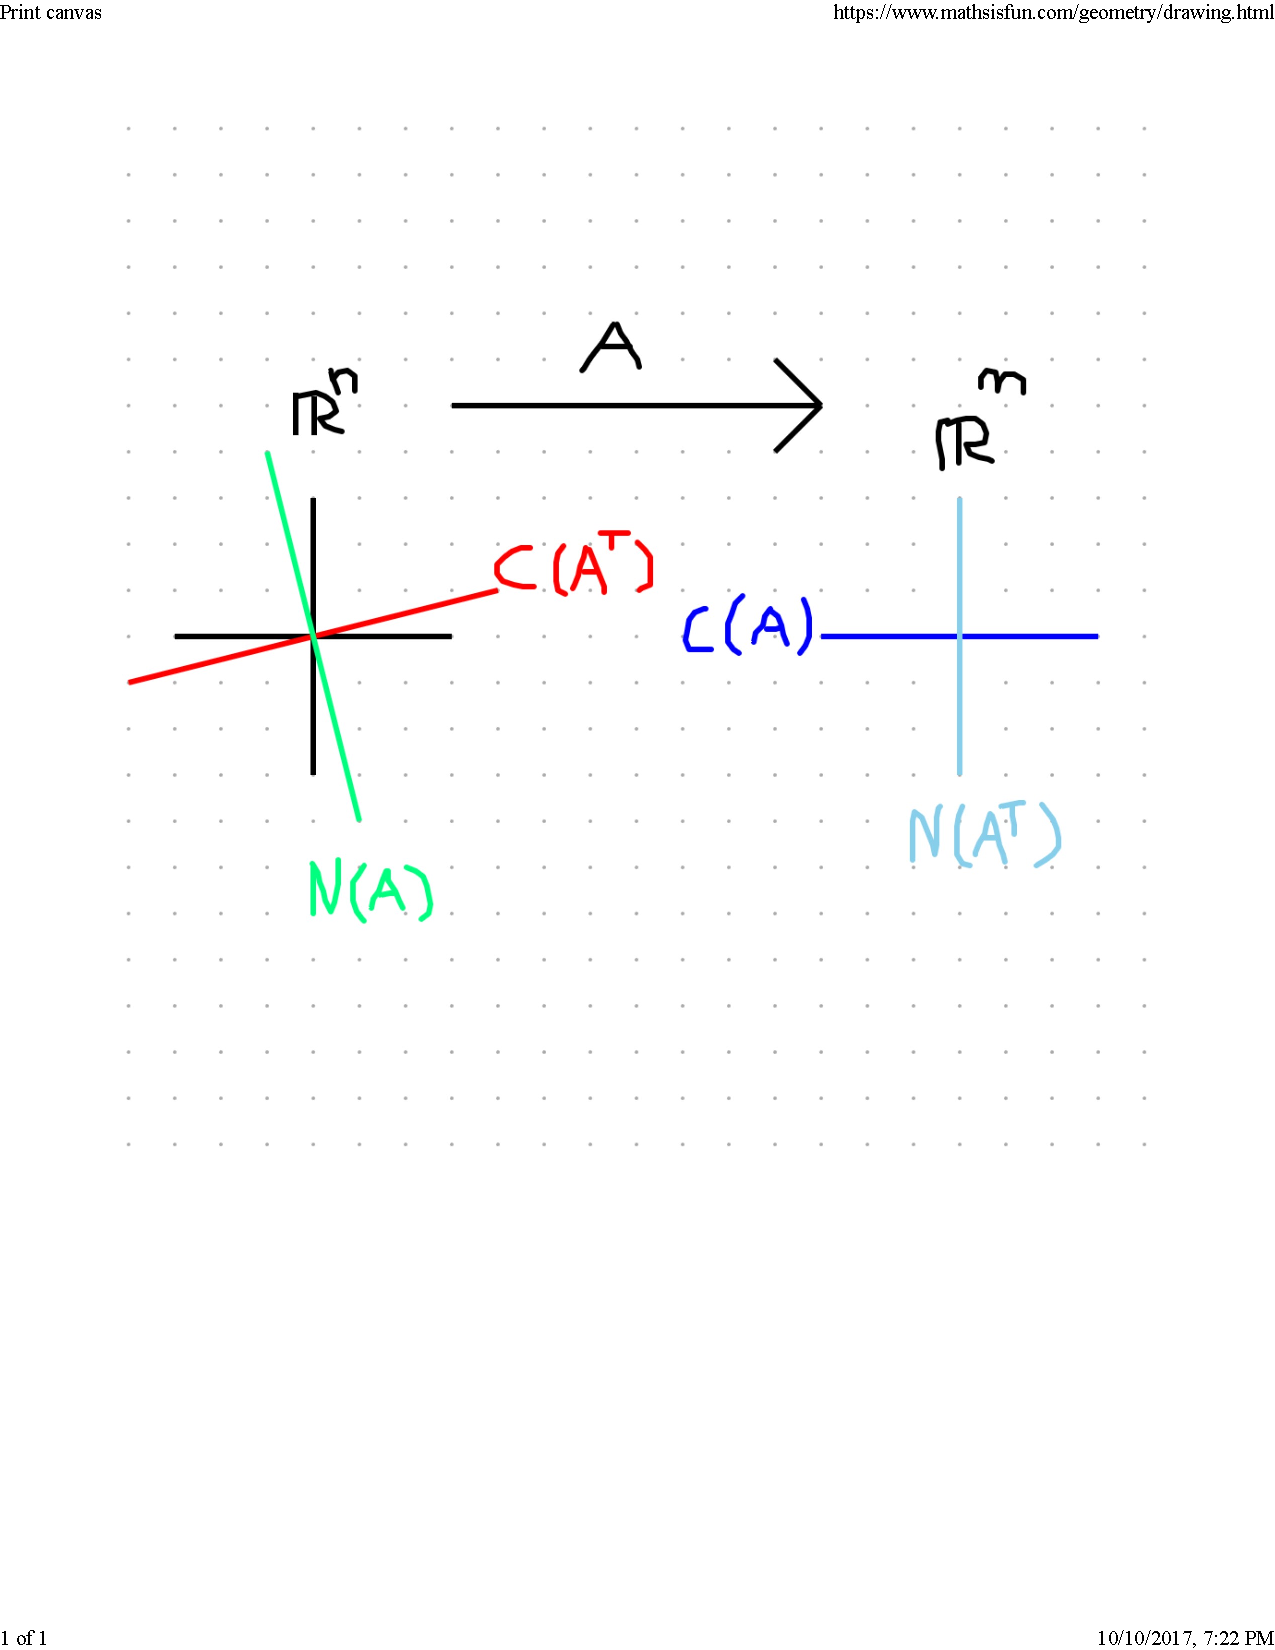
\includegraphics[scale=0.5]{poorly-drawn-graphs.pdf}
\end{center}

\item[S7)] Using one of our methods for matrix multiplication and the product $AA^{-1}$, explain and show that the first column of $A^{-1}$ is orthogonal to the space spanned by some rows of $A$.  (You will need to determine all rows that the first column is orthogonal to.)

\textit{Solution.} $AA^{-1}=I$. Recall the dot product method for multiplying matrices, and that when a dot product results in 0, the two vectors dotted together are orthogonal. Since the first column of $A$ dotted with any column of $A^{-1}$ is zero with the exception of the first column of $A^{-1}$, the first column of $A^{-1}$ is orthogonal to the space spanned by all rows of $A$ except the first row of $A$.

\end{itemize}
\end{document}

$\vec{u}=\left[\begin{array}{c} 1 \\ 0\end{array}\right]$

$\left[\begin{array}{cc}  & \\  & \end{array}\right]$

$\left[\begin{array}{ccc}  &  & \\  &  & \\ & & \end{array}\right]$

CREATE VECTOR
$\vec{u}=\left[\begin{array}{c} 1 \\ 0\end{array}\right]$

CREATE EQUATION
$A = \begin{align}{cc}
 1 & 2\\
3 & 4
\end{align}$

CREATE EQUATION
\begin{equation}
y=x
\end{equation}

CREATE SYSTEM OF EQUATIONS
\begin{align}
y&=x\\
y&=x
\end{equation}

